\section{Discriminative ve Generative Modeller}
Discriminative modeller, doğrudan belirli bir sınıflandırma görevi için doğrudan koşullu dağılımları modellemeye odaklanır. Sınıflandırma veya regresyon gibi belirli bir çıktıya doğru haritalama yaparlar. Örnek olarak, lojistik regresyon, destek vektör makineleri, karar ağaçları ve derin öğrenme ağları gibi modeller verilebilir. Discriminative modeller, veri setinin verilerle etiketlendiği durumlarda özellikle kullanışlıdır. Discriminative modeller, genellikle daha yüksek doğruluk ve daha düşük hesaplama maliyeti sağlar. Verilerin dağılımı hakkında bilgi vermezler. Yeni veri üretmezler.

Generative modeller, veri setinin ardında yatan veri dağılımını modellemeye odaklanır. Bu modeller, veri setinin oluşturulma sürecini anlamak ve veri seti içindeki verileri üretmek için kullanılabilir. Örnek olarak, naif bay, gizli markov modeleri ve generative adversarial networks (GANs) gibi modeller verilebilir. Generative modeller, veri setinin etiketlenmediği veya eksik olduğu durumlarda kullanışlıdır, çünkü veri setinin yapısını ve içeriğini daha iyi anlayabilirler. Generative modeller, yeni veri örnekleri üretmek, eksik verileri tamamlamak veya veri setinin oluşturulma sürecini modellemek için kullanılabilirler. Genellikle daha yavaş ve daha fazla veriye ihtiyaç duyarlar.

\begin{figure}[h]
    \centering
    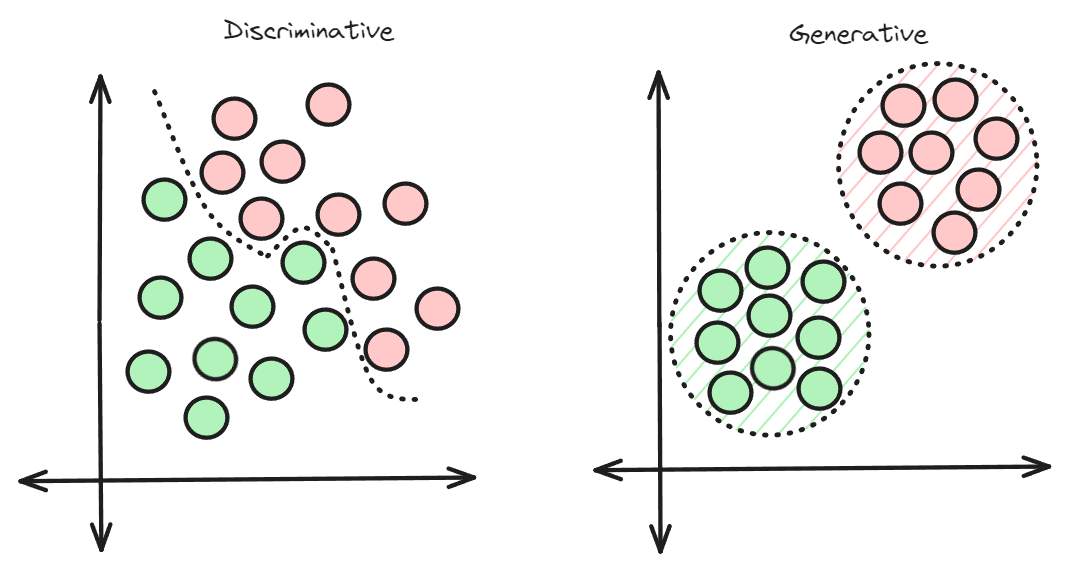
\includegraphics[width=1\textwidth]{images/discriminative_vs_generative_models.png}
    \caption{Discriminative ve Generative Modeller}
    \label{fig:enter-label}
\end{figure}

\newpage